\inputencoding{utf8}
\section{Categorization-based Concept}
\label{sec:cbc} 

Usually, requirements provided by stakeholders have poor structure and ambiguous description of a designed system. This can possibly lead to misunderstandings from developers or reviewers. Furthermore, a poor readability of requirements might result in mistakes within system design or time increasing for their review. All these points indicate a low quality. 

In order to improve quality of requirements and prevent mentioned problems, requirements should be structured and formalized to become more exact. Here we claim, that \cbc aims this purpose providing a method for arranging requirements in a consistent structure.

The idea behind \cc arises from common requirements categorization and goes ahead forming a structure of textual requirements. Requirements are categorized by their characteristics. Therefore, one or more categories can be attached to a single requirement, depending on the requirement's composition. The number of applied categories increases with rising complexity of the considered requirement. That implies, a requirement with a range of categories should be splitted into several simplified requirements with less number of attached categories, if it is possible with respect to context.

The user can define, which categories correspond to each requirement. Moreover, \cc provides a certain degree of freedom for the user to choose a granularity of every attached category. In other words, the user makes a decision on how detailed the requirements should be considered and categorized. After an analysis of the whole scope of requirements, every requirement should be categorized.  

The output of this procedure is structured and more consistent requirements with attached set of corresponding categories. This set constitutes a new artifact in system development process, that represents a full structure of the requirements. Such structured requirements are more precise and unambiguous. Thanks to that the reviewing process becomes easier and more accurate; risk of mistakes in system design declines due to better legibility of requirements. We can conclude, that quality of requirements increases by applying \cbc.

Additionally, the idea of the \cc is general and allows a user to be independent from specific tools. It can be applied within already known for a user chain of tools and thereby, save costs and time for a project realization, instead of training employees for new extra tools. 

\subsection{\cbc in \autof}
\label{sec:cbcinaf}

\cc has been implemented in \autof. In \af requirements categorization incarnates so called \asp (templates for requirements characteristics, which represent requirements' categories).   

In \af eight \asp have been created, which are depicted in \autoref{fig:fig_aspects}. 

\begin{itemize}
\item	\textit{Timing aspect} - the requirement refers to timing constraints
\item	\textit{Signal aspect} - the requirement defines a signal, its type and its range
\item	\textit{Parameter definition aspect} - the requirement defines a parametric value. This allows to re-use the requirement by changing the value of the parameter
\item\textit{Safety level aspect} - the requirement defines a safety level of the system
\item	\textit{Mode aspect} - the requirement defines an operational state of system e.g. active/inactive mode.
\item	\textit{Design choice aspect} - the requirement was derived from a design choice of the software developer
\item	\textit{Functional aspect}- the requirement specifies a particular behavior by relating inputs and outputs
\item	\textit{Temporal property aspect} - the requirement defines a property expressed by temporal patterns
\end{itemize}

\begin{figure}[!t]
\centering
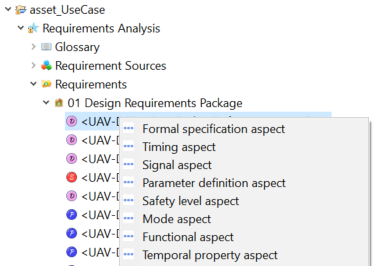
\includegraphics[width=2in]{asset_aspects.png}
\caption{List of \textit{aspects} in \autof}
\label{fig:fig_aspects}
\end{figure}

However, the number of \asp can vary with respect to a context of project and needs of requirements engineer/ reviewer. \textit{Aspects} can be applied to system requirements from initial stage of the development process, from requirements elicitation. \textit{Aspects} form a structure of the analyzed requirements tagging them. \autoref{fig:pd_aspect_tag} presents a view of a textual requirement with assigned \textit{Parameter definition aspect}.
\begin{figure}[!t]
\centering
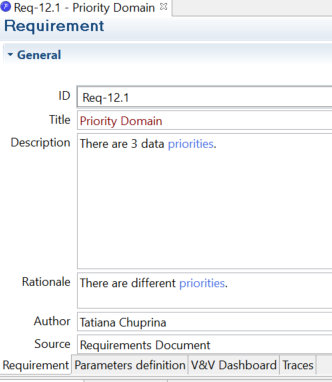
\includegraphics[width=1.6in]{param_aspect_tag.png}
\caption{Requirement with Assigned \textit{Parameter definition aspect} in \autof}
\label{fig:pd_aspect_tag}
\end{figure}

As it was mentioned above, every aspect provides a template for requirement's main characteristics. The templates collect meta-data of requirements. For instance, \autoref{fig:pd_aspect_view} shows a view of \textit{Parameter definition aspect} template attached to a corresponding requirement. 
\begin{figure}[!t]
\centering
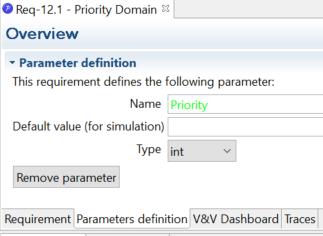
\includegraphics[width=1.6in]{aspect_view.png}
\caption{\textit{Parameter definition aspect} template in \autof}
\label{fig:pd_aspect_view}
\end{figure}

As it is shown in \autoref{fig:pd_aspect_view}, the aspect template includes information from tagged requirement, thereby binding the aspect and the requirement together. Data captured in aspects' templates depends on the granularity of the applied category (aspect), chosen by the \cc user.  Furthermore, the structured requirements with assigned \asp appear as an input for development and reviewing processes. This means, that \asp link artifacts of these processes (e.g system architectures, low-level requirements (LLR), review results, etc.) supporting traceability between them; contribute in mapping requirements into system design. 

In addition, it is easier to check structured requirements.

Summing up all statements from above, \asp based on \cbc, facilitate in increasing quality of requirements. 

Let us consider \cc with the ”Router” use case, which was inspired by an industrial project being conducted together with Airbus and Fortiss. 
